%% ------------------------------------------------------------------------ %%
\documentclass[draft, 12pt]{article}
\usepackage[english]{babel}
\usepackage[final]{graphicx}
\graphicspath{ {figures/} }
\DeclareGraphicsExtensions{.png}


\title{Seismic parameter estimation and the Canadian crust}
\author{Ben Postlethwaite}

%% ------------------------------------------------------------------------ %%
\begin{document}


%% ------------------------------------------------------------------------ %%
\begin{abstract}
   It has been suggested that processes driving crustal formation in the Archean and Proterozoic were dissimilar and produced crusts with unique bulk properties and average thicknesses. Existing models based on fractionating mantle composition or evolving mantle convection require accurate estimates of the geological and geophysical properties of crustal provinces to better understand the details of early continental formation (R. Durrheim, W. Mooney, 1991). Fifteen years of publicly accessible teleseismic data from all available Canadian seismic stations are binned in horizontal slowness and deconvolved into receiver functions. We apply a new stacking method (Bostock and Kumar, 2010) to retrieve estimates of bulk crustal velocities (Vp, Vs) and thickness H from these data under the assumption of 1-D structure. Bootstrap error analysis is performed for each station dataset and results are compared to the results produced from alternate methods (Zhu and Kanamori, 2000). Cross-analyzing these results with the mineral and rock seismic property database of Christensen (1996) will afford improved constraints on bulk geological composition of the Canadian landmass. These results will be used to evaluate competing models of early crustal formation.
\end{abstract}

%% ------------------------------------------------------------------------ %%

%% ------------------------------------------------------------------------ %%
%% -----------------------------------------------%%
\section{Introduction}
(Article text here)
\subsection{Overview}
(Overview here)
\subsection{Geological Background}
(Geological background here)

%% -----------------------------------------------%%
\section{Data and method}
   Seismic data utilized in this study come from 343 stations across Canada from all available networks. Of these stations 146 are of sufficient quality to be useful for study. All stations are broadband with data selected between the years 2000 and 2012, for a total of more than 700 earthquake sources. All teleseismic events outside of the 30 to 100 degrees of epicentral distance are removed before processing. Data is selected for reasonable signal to noise ratioand sufficient impulsiveness that arrival times can be calculated. All data is analyzed using receiver function methods, an approach which has been widely employed over many years to investigate the earths structure.

   Two derivations of receiver function analysis have been used in this study, one well tested stacking approach and the other a recent method that has not yet been employed at scale. Both methods rely on the fact that the incoming S-wave contains energy from the direct arrival as well as reflected phases resulting from sharp velocity contrasts. Deconvolution of the P-wave energy arrival, used as an estimate for the source function, from the S-wave signal produces a Green's function with energy peaks at the times of the main and reflected arrivals. For better separation of P and S wave energy all components are rotated into radial and transverse dimensions and transformed into P, SV and SH components with a wave field decomposition transfer matrix (Bostock, 1998).
   Deconvolution is performed by minimizing the general cross validation function $GCV(\delta)$ where $\delta$ is used the regularizer (Bostock, 1998; Golub et al., 1979). This method is an $L_2$ frequency domain deconvolution which performs quickly and makes no assumptions on the noise in the data. All deconvolved signals are filtered between 0.04hz and 3.0hz and are stacked with weights $w_1=0.5$, $w_1=0.3$, $w_1=0.2$ for the Ps, PpPs and PpSs phases respectively. Error calculations are performed with bootstrap resampling by rerunning the processing with randomly chosen receiver functions - allowing multiples - 1024 times. The error is obtained by taking the standard deviation of the results.

\subsection{Vp/Vs method}
   A well tested approach for calculating $R=\frac{V_P}{V_S}$ and $H$ was employed by Zhu and Kanamori (2000). After deconvolution the signals are stacked and a gridsearch is performed using the travel time equations for different values of $R$ and $H$ and a spectrum of slowness. For each parameter combination the travel time functions output estimates for the differential arrival time of the S-component main and reflected phases. These times are used to pick the energy in each receiver function - with the large amplitudes at arrivals stacking to provide an estimate for the optimal parameter estimation.

\subsection{Vp method}
   The stacking approach outlined above provides estimates for the parameters $R=\frac{V_P}{V_S}$ as well as crustal thickness $H$ - which gives the depth of the Moho. A method which estimates $V_P$ and $V_S$ separately (Bostock, 2010) is also employed for select stations. This method makes use of the fact the dependence on $H$ in the travel time equations can be removed if we divide the reflected phases by the main arrival.
$$ t_{Pps}(p_i) = \frac{ \sqrt{R^2-p_i^2V_P^2} + \sqrt{1-p_i^2V_P^2} } {\sqrt{R^2-p_i^2V_P^2} + \sqrt{1-p_i^2V_P^2} } t_{Ps}(p_i) $$
$$ t_{Pss}(p_i) = \frac{2\sqrt{R^2-p_i^2V_P^2}} {\sqrt{R^2-p_i^2V_P^2} + \sqrt{1-p_i^2V_P^2} } t_{Ps}(p_i) $$
This has the advantage that no assumptions on $V_P$ are necessary to perform the gridsearch and stack. A similar stacking method as the Zhu and Kanamori approach may be employed for $t_{Pps}$ and $t_{Pss}$ as long as an estimate for $t_{Ps}$ exists. With estimates for $R$ and $V_P$ a simple line search along $H$ can be made using all three undivided travel time equations.

Several methods for choosing $t_{Ps}$ are available. Direct arrival $t_{Ps}$ should contain the largest fraction of energy out of the other phases and the moveout, depending on Moho depth, should be in the order of 3 to 6 seconds. Given this it is trivial to define a window and select the time corripsonding to maximum amplitude. Another approach is to use max amplitude estimates as data in a non-linear optimization to find the $R$, $V_P$, and $H$ which minimizes the residual between $t_{Ps}$ and the data. The travel time equations are twice-differentiable so the quadratically convergent Newton's method may be employed. This approach has the advantage that noise leading to poor maximum amplitude picks are effectively collapsed onto the curve corrisponding to the travel time function. A third approach which offers picks along a travel time curve but better stability than the non-linear method is to perform a gridsearch with all three travel time functions, a full Kanamori stack. With the best estimates for $R$ and $H$ the $t_{Ps}$ function can be found and used as input into the Bostock method. The trade-off is that the requirement for an initial $V_P$ estimate for the initial stack introduces secondary $V_P$ dependence into the system.

\subsection{Vp database}
   Accompanying the processed estimates outlines above are data from controlled source experiments collected and compiled by external sources. The data was compiled by Mooney (personal communication, 2012).


%% -----------------------------------------------%%
\section{Results}
As regional studies exist which utilize similar methods and have corrisponding parameter estimates for some of the stations used in this study it is possilbe to directly compare values to those previously published. A comprehensive study in the Hudson Bay region of the Canadian Shield (Thomson et. al., 2010) uses an approach similar to the Zhu and Kanamori method provides estimates for $H$ and $R=/frac{V_P}{V_S}$ for 35 stations. 5 stations with $R$ estimates above 1.8 are removed due to the uncertainty surrounding these high values. Both datasets are plotted in Figure~\ref{fig:thompsonComp}. The Pearson correlation coefficient between these datasets is 0.49. [Compare this value to uncertainty / deviation in the data? ].

Directly comparing $V_P$ estimates processed with the MB algorithm is not possible as this method has not been employed in publication. However, comparisons can be made to active source records for experiments within close proximity to a given seismic station (Figure~ \ref{fig:activeComp}. The correlation between these datasets is 0.235. [This is low, explain here?]. Another method of determining the reliability of estimates is to check the $/frac{V_P}{V_S}$ ratio taken from the Kanamori approach to the $/frac{V_P}{V_S}$ value computed from the MB approach. These values, working with the same data, preprocessed using the same methods and tools should be equal. Selecting only those stations who have an error of less than +/-0.05 $R$, 132 stations, we get a correlation of 0.57. Reducing the error tolerance and selecting stations with less than +/-0.01 $R$, leaving 31 of the cleanest stations, we get a correlation coefficient of 0.95.

\begin{figure}
  \centering
    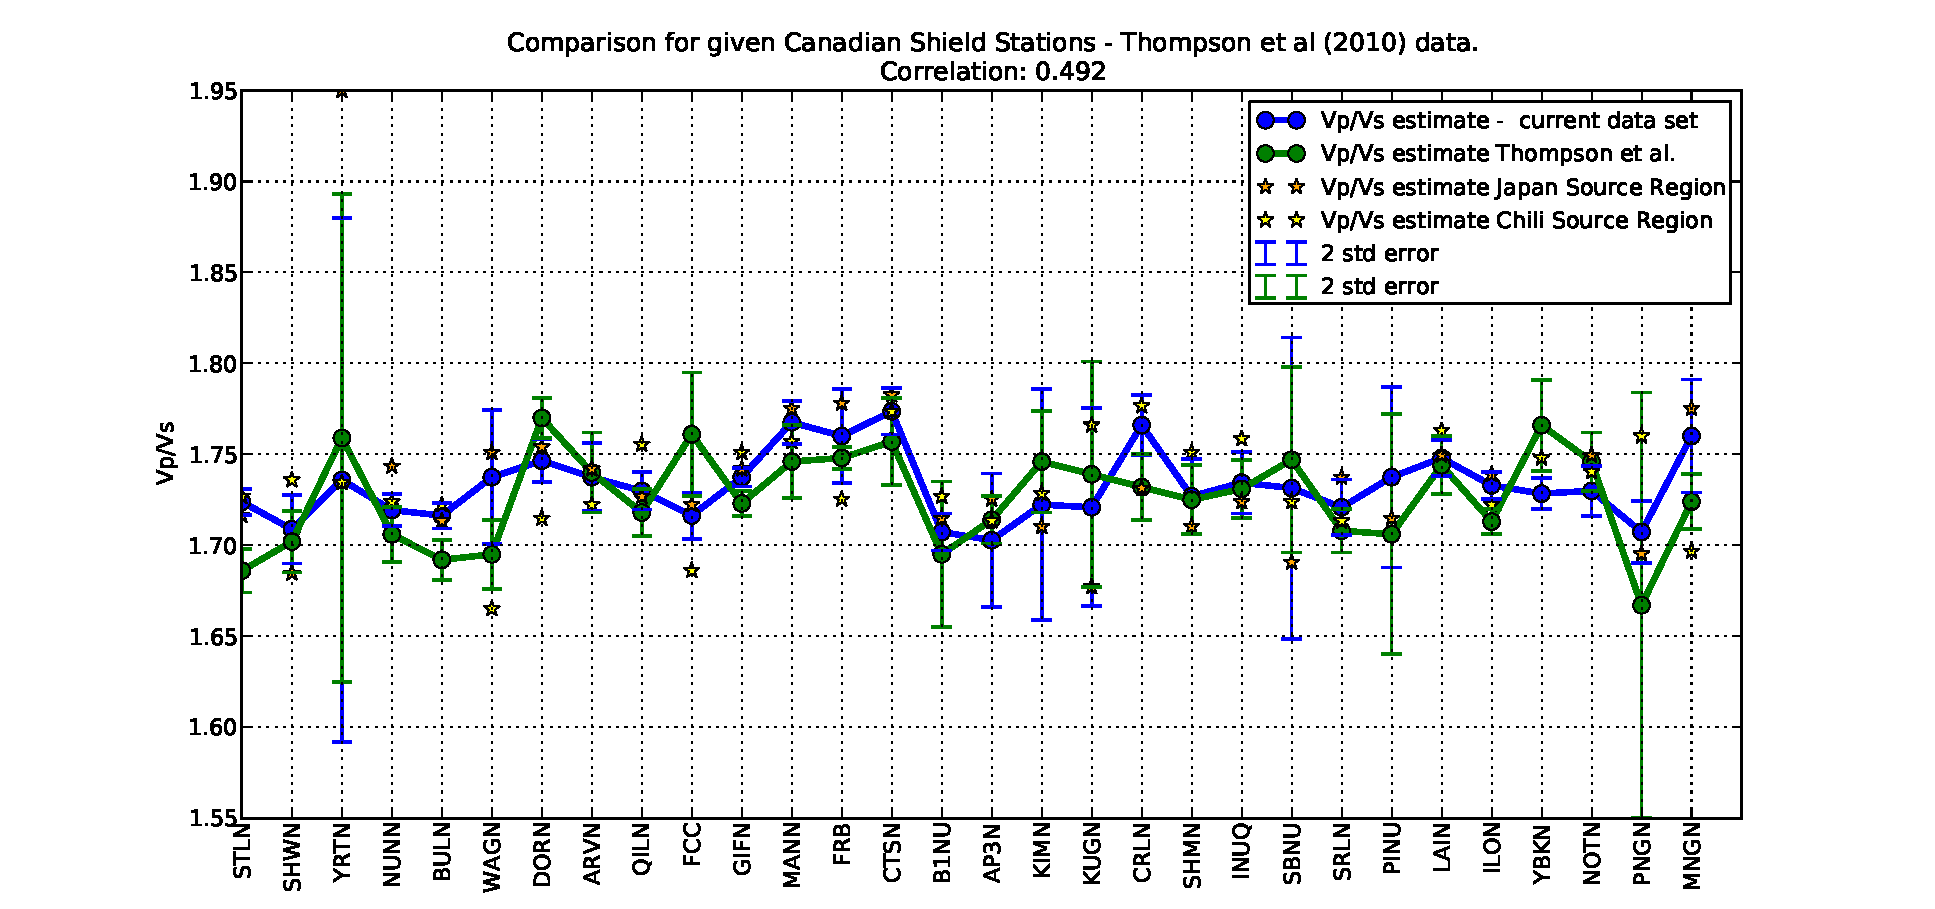
\includegraphics[width=\textwidth]{thompsonComparison}
  \caption{Comparison of $\frac{V_P}{V_R}$ data processed for this study with data from Thomspson et. al. (2010).}
  \label{fig:thompsonComp}
\end{figure}

\begin{figure}
  \centering
    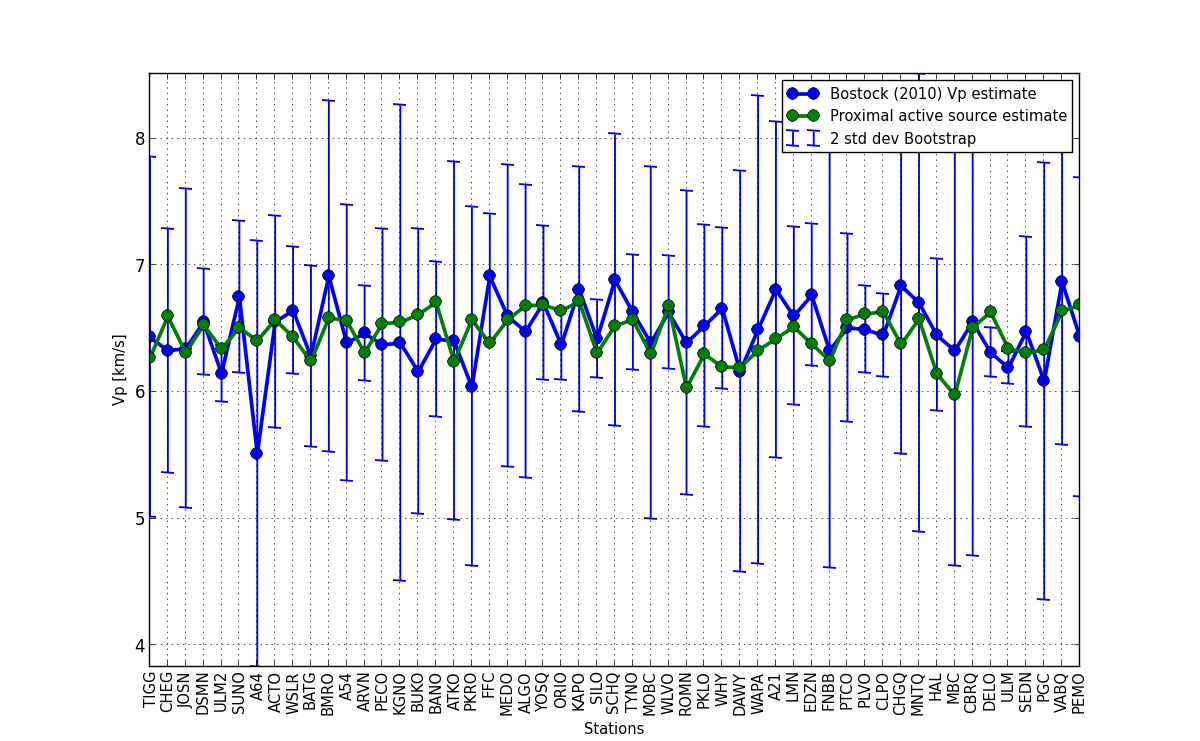
\includegraphics[width=\textwidth]{activeSourceComparison}
  \caption{Comparison of $V_P$ estimates from the MB algorithm with active source $V_P$ recordings. Stations selected if active source experiment locations within 1 degree of latitude / longtitude.}
  \label{fig:activeComp}
\end{figure}


  The preliminary interrogation of the data set yields the observation that the bulk Canadian crust is more felsic than originally anticipated. Previous experiments show crustal averages of 0.265 (Christensen and Mooney, 1995) or have averages of at least 0.27 for shields, platforms and paleozoic units (Zandt and Ammon, 1995). The weighted average for this data set shows a Poisson' ratio of 0.258 with the weighting for each station given by the calculation of the stations inverse Voronoi cell area. At the regional scale we have values of 0.251. 0.254, 0.260, 0.275 for the Churchill, Superior, Slave and Grenville Provinces Poisson's ratios respectively. Most of the Canadian Shield stations also appear to have low Poisson values with the exception of the Grenville Province which has a high Poisson Ratio of 0.275.

  The data bears out earlier results showing Proterozoic crust to have a higher Poisson's ratio than Archean crust, likely the result of a more mafic composition. The increased crustal thickness of Proterozoic crust is clearly seen in the active source data while it not visible in data from processed seismic stations. The most likely reason for not seeing the signal of thicker crust in the station data is owing to poor station coverage in Proterozoic regions.

  Further work on the Bostock-Kumar stacking approach is warranted from a look at the cleanest stations. Before it can be employed in large scale analysis additional denoising methods or alternative deconvolution techniques will need to be investigated to reduce the noise in the data.



%% -----------------------------------------------%%
\section{Discussion}
\subsection{Canada}
<Discussion on larger - Canada wide - regions>
\subsection{Slave Province}
<Discussion on Slave Province>

%% -----------------------------------------------%%
\section{Conclusions}
<Conclusions here>

%% ------------------------------------------------------------------------ %%


% AGU does not want a .bib or a .bbl file. Please copy in the contents of your .bbl file here.

\begin{thebibliography}{}


\end{thebibliography}

%Reference citation examples:

%...as shown by \textit{Kilby} [2008].
%...as shown by {\textit  {Lewin}} [1976], {\textit  {Carson}} [1986], {\textit  {Bartholdy and Billi}} [2002], and {\textit  {Rinaldi}} [2003].
%...has been shown [\textit{Kilby et al.}, 2008].
%...has been shown [{\textit  {Lewin}}, 1976; {\textit  {Carson}}, 1986; {\textit  {Bartholdy and Billi}}, 2002; {\textit  {Rinaldi}}, 2003].
%...has been shown [e.g., {\textit  {Lewin}}, 1976; {\textit  {Carson}}, 1986; {\textit  {Bartholdy and Billi}}, 2002; {\textit  {Rinaldi}}, 2003].



%...as shown by \citet{jskilby}.
%...as shown by \citet{lewin76}, \citet{carson86}, \citet{bartoldy02}, and \citet{rinaldi03}.
%...has been shown \citep{jskilbye}.
%...has been shown \citep{lewin76,carson86,bartoldy02,rinaldi03}.
%...has been shown \citep [e.g.,][]{lewin76,carson86,bartoldy02,rinaldi03}.
%
% Please use ONLY \citet and \citep for reference citations.
% DO NOT use other cite commands (e.g., \cite, \citeyear, \nocite, \citealp, etc.).

%% ------------------------------------------------------------------------ %%


\end{document}

%% ------------------------------------------------------------------------ %%


M. G. Bostock, M. R. Kumar, 2010. Bias in seismic estimates of crustal properties, Geophys. J. Int., 182, 403-407.
N. I. Christensen, 1996. Poisson's ratio and crustal seismology, J. Geophys. Res., 101, 3139–3156,
R. J. Durrheim, W. D. Mooney, 1991. Archean and Proterozoic crustal evolution, Geology, 19, 606-609.
W. D. Mooney. 2012. Personal communication. Compiled GSC active source data for the Canada.
D.A. Thompson, I.D. Bastow, G. Helffrich, J-M. Kendall, J. Wookey, D.B. Snyder, D.W. Eaton, 2010. Precambrian crustal evolution: Seismic constraints from the Canadian Shield, Earth and Planetary Science Letters, Volume 297, Issues 3–4, 1 September 2010, Pages 655–666
L. Zhu, H. Kanamori, 2000. Moho depth variation in Southern California from teleseismic receiver functions, J. Geophys Res, 105, 2969-2980.
G. Zandt, C. J. Ammon, 1995. Continental crust composition constrained by measurements of crustal Poisson's ratio, Nature, 374, 152-154.

More Information and Advice:


%
%  SECTION HEADS
%
%% ------------------------------------------------------------------------ %%

% Capitalize the first letter of each word (except for
% prepositions, conjunctions, and articles that are
% three or fewer letters).

% AGU follows standard outline style; therefore, there cannot be a section 1 without
% a section 2, or a section 2.3.1 without a section 2.3.2.
% Please make sure your section numbers are balanced.
% ---------------
% Level 1 head
%
% Use the \section{} command to identify level 1 heads;
% type the appropriate head wording between the curly
% brackets, as shown below.
%
%An example:
%\section{Level 1 Head: Introduction}
%
% ---------------
% Level 2 head
%
% Use the \subsection{} command to identify level 2 heads.
%An example:
%\subsection{Level 2 Head}
%
% ---------------
% Level 3 head
%
% Use the \subsubsection{} command to identify level 3 heads
%An example:
%\subsubsection{Level 3 Head}
%
%---------------
% Level 4 head
%
% Use the \subsubsubsection{} command to identify level 3 heads
% An example:
%\subsubsubsection{Level 4 Head} An example.
%
%% ------------------------------------------------------------------------ %%
%
%  IN-TEXT LISTS
%
%% ------------------------------------------------------------------------ %%
%
% Do not use bulleted lists; enumerated lists are okay.
% \begin{enumerate}
% \item
% \item
% \item
% \end{enumerate}
%
%% ------------------------------------------------------------------------ %%
%
%  EQUATIONS
%
%% ------------------------------------------------------------------------ %%

% Single-line equations are centered.
% Equation arrays will appear left-aligned.

Math coded inside display math mode \[ ...\]
 will not be numbered, e.g.,:
 \[ x^2=y^2 + z^2\]

 Math coded inside \begin{equation} and \end{equation} will
 be automatically numbered, e.g.,:
 \begin{equation}
 x^2=y^2 + z^2
 \end{equation}

% IF YOU HAVE MULTI-LINE EQUATIONS, PLEASE
% BREAK THE EQUATIONS INTO TWO OR MORE LINES
% OF SINGLE COLUMN WIDTH (20 pc, 8.3 cm)
% using double backslashes (\\).

% To create multiline equations, use the
% \begin{eqnarray} and \end{eqnarray} environment
% as demonstrated below.
\begin{eqnarray}
  x_{1} & = & (x - x_{0}) \cos \Theta \nonumber \\
        && + (y - y_{0}) \sin \Theta  \nonumber \\
  y_{1} & = & -(x - x_{0}) \sin \Theta \nonumber \\
        && + (y - y_{0}) \cos \Theta.
\end{eqnarray}

%If you don't want an equation number, use the star form:
%\begin{eqnarray*}...\end{eqnarray*}

% Break each line at a sign of operation
% (+, -, etc.) if possible, with the sign of operation
% on the new line.

% Indent second and subsequent lines to align with
% the first character following the equal sign on the
% first line.

% Use an \hspace{} command to insert horizontal space
% into your equation if necessary. Place an appropriate
% unit of measure between the curly braces, e.g.
% \hspace{1in}; you may have to experiment to achieve
% the correct amount of space.


%% ------------------------------------------------------------------------ %%
%
%  EQUATION NUMBERING: COUNTER
%
%% ------------------------------------------------------------------------ %%

% You may change equation numbering by resetting
% the equation counter or by explicitly numbering
% an equation.

% To explicitly number an equation, type \eqnum{}
% (with the desired number between the brackets)
% after the \begin{equation} or \begin{eqnarray}
% command.  The \eqnum{} command will affect only
% the equation it appears with; LaTeX will number
% any equations appearing later in the manuscript
% according to the equation counter.
%

% If you have a multiline equation that needs only
% one equation number, use a \nonumber command in
% front of the double backslashes (\\) as shown in
% the multiline equation above.

%% ------------------------------------------------------------------------ %%
%
%  LANDSCAPE/SIDEWAYS FIGURE AND TABLE EXAMPLES
%
%% ------------------------------------------------------------------------ %%
%
% For figures, add \usepackage{lscape} to the file and the landscape.sty style file
% to the paper folder.
%
% \begin{figure*}[p]
% \begin{landscapefigure*}
% Illustration here.
% \caption{caption here}
% \end{landscapefigure*}
% \end{figure*}
%
% For tables, add \usepackage{rotating} to the paper and add the rotating.sty file to the folder.
%
% AGU prefers the use of {sidewaystable} over {landscapetable} as it causes fewer problems.
%
% \begin{sidewaystable}
% \caption{}
% \begin{tabular}
% Table layout here.
% \end{tabular}
% \end{sidewaystable}
%
%
